

\subsection{Analyse}

    \textbf{ Diagramme de cas d'utilisation "G\'{e}rer un membre"}
    \begin{figure}[H]
    \center
    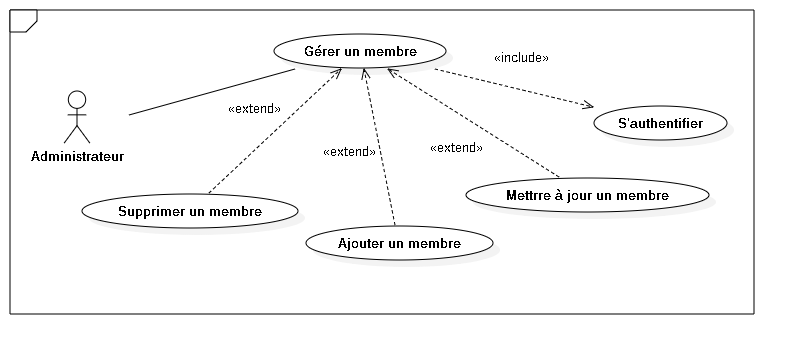
\includegraphics[width=13cm,height=8cm]{./figures/ucM.png}
    \caption{G\'{e}rer un membre.}

    \end{figure}

\subsection{Conception}

Le diagramme de s\'{e}quence indique l'interaction entre plusieurs acteurs
afin d'expliquer le d\'{e}roulement des diff\'{e}rents sc\'{e}nario entre les diff\'{e}rents
\'{e}l\'{e}ments du projet.

\subsubsection{Le sc\'{e}nario \guillemotleft{} Cr\'{e}ation d'un membre \guillemotright{}}

Le diagramme de s\'{e}quence \guillemotleft{} Ajout d'une t\^{a}che \guillemotright{} pr\'{e}sente le s\'{e}quencement
des interactions entre Administrateur, Application et Base de donn\'{e}es (BD).


\subsection{Sch\'{e}ma}

\textbf{La table \guillemotleft{} members \guillemotright{}}

\begin{table}

\begin{tabular}{|l|l|l|l|l|l|}
\hline
Field        & Type         & Null & Key & Default            & Extra            \\
\hline
id           & int(11)      & NO   & PRI & NULL               & auto\_increment  \\
\hline
login        & varchar(30)  & YES  &     & NULL               &                  \\
\hline
password     & varchar(15)  & YES  &     & NULL               &                  \\
\hline
firstname    & varchar(50)  & YES  &     & NULL               &                  \\
\hline
lastname     & varchar(30)  & YES  &     & NULL               &                  \\
\hline
email        & varchar(100) & YES  &     & NULL               &                  \\
\hline
hiredate     & datetime     & YES  &     & CURRENT\_TIMESTAMP &                  \\
\hline
color        & varchar(6)   & YES  &     & NULL               &                  \\
\hline
projects\_id & int(11)      & YES  & MUL & NULL               &                  \\
\hline
pname        & varchar(50)  & YES  &     & NULL               &                  \\
\hline
\end{tabular}
\centering
 \caption {Members.}
\end{table}


\subsection{Test}

Dans ce premier sprint, nous testons la fonctionnalit\'{e}
« Gestion des membres» qui affiche, ajoute,
supprime les membres de la base de donn\'{e}es.
Ci-dessus nous ajoutons des captures \'{e}cran du sprint r\'{e}alis\'{e}.

\bigskip
\bigskip

Lors de la cr\'{e}ation d'un utilisateur , un email contenant son mot de passe lui
sera envoy\'{e}, ainsi si on modifie les param\'{e}tres d'utilisateur , un nouveeau
mot de passe lui sera envoy\'{e} sur la nouvelle addresse email .

\bigskip
\bigskip

\FloatBarrier
\begin{figure}[H]
\center
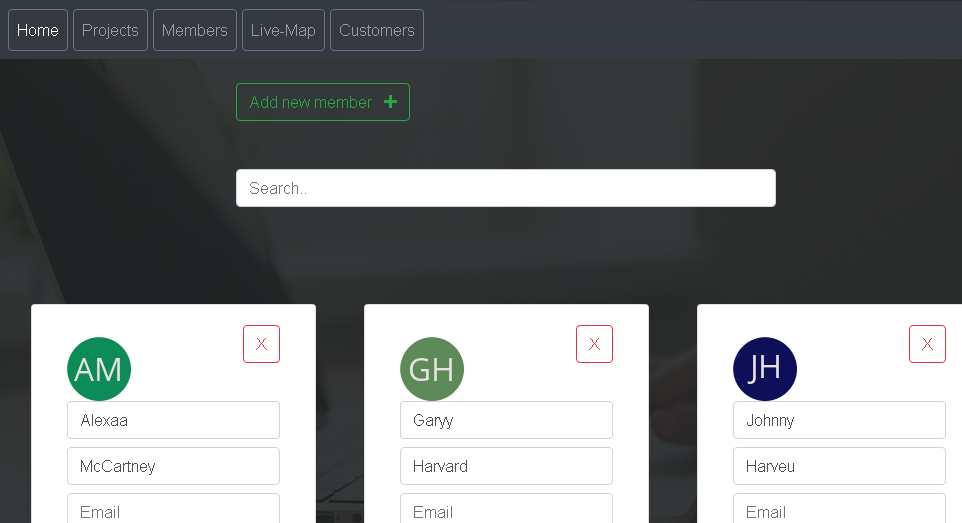
\includegraphics[width=11cm,height=7cm]{./figures/pres/mm1.png}
\caption{Gestion des membres.1.}
\end{figure}
\FloatBarrier



\FloatBarrier
\begin{figure}[H]
\center
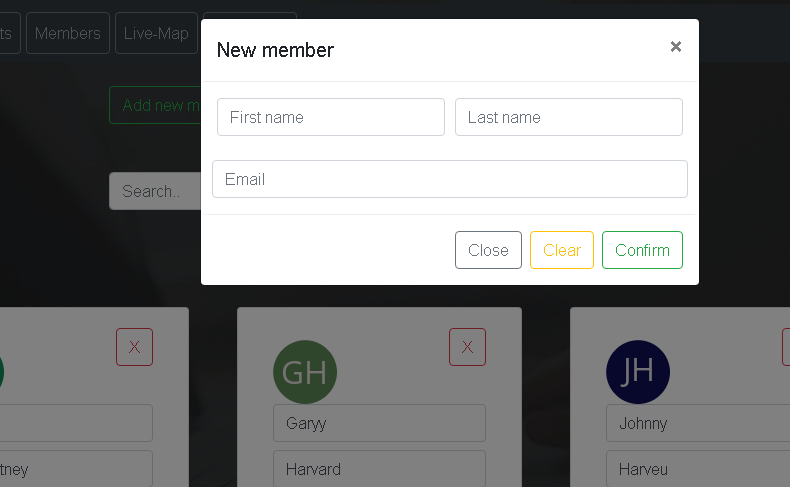
\includegraphics[width=11cm,height=7cm]{./figures/pres/mm2.png}
\caption{Gestion des membres.2.}
\end{figure}
\FloatBarrier


\FloatBarrier
\begin{figure}[H]
\center
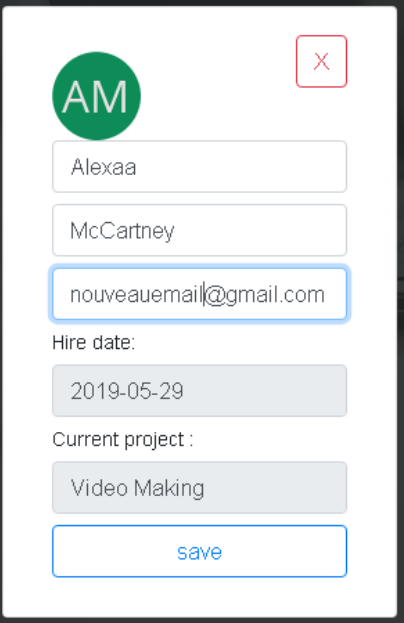
\includegraphics[width=11cm,height=7cm]{./figures/pres/mm3.png}
\caption{Gestion des membres.3.}
\end{figure}
\FloatBarrier

